%\fill[top color=red!25, bottom color=blue!25, draw=black] (0,0) rectangle ++(\R,\L);
%\draw[fill=blue!25] (0,0) rectangle ++(\R,-\HX);
%\draw[fill=red!25] (0,\L) rectangle ++(\R,\HX);
%
%\foreach \z [evaluate=\z] in {0,...,4}{
%	\foreach \r [evaluate=\r as \num using int(\r+1 + 3*\z)] in {0,...,2}{
%		\draw ({-(\R-.4)/2*\r+\R-.2},{\z*(1+\L)/4-.5}) node(n\z\r){\num};
%}}
%
%\draw (n40.south east) node [right]{AHX};
%\draw (n00.north east) node[right]{CHX};
%\draw (n01.south) node [below]{\shortstack{ $\downarrow$ \\Source acoustique principale}};
%
%\draw (0,\L+2*\HX+\spy) node [anchor=west]{\textbf{(c)} \texttt{V1}};

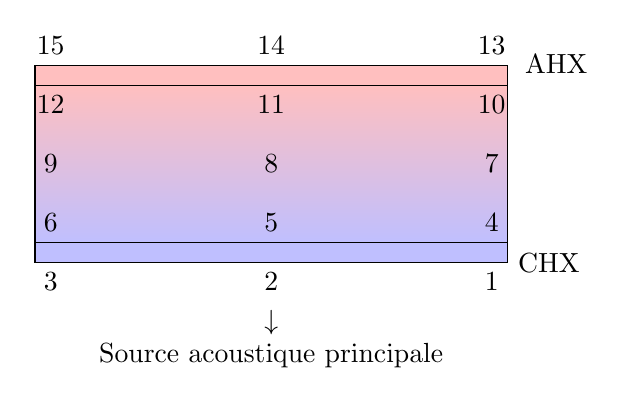
\begin{tikzpicture}

%    \def\lenreg{2};
%    \def\diam{3};
    \def\spy{2};
    \def\xdist{8cm};
    \def\ydist{-7cm};
%    \def\persp{20};
%    
%    \def\LX{1};
%    \def\LY{2};
%    \def\CoreX{1.5};
%    \def\CoreY{.9*\LY};
%    

	\def\L{2};
	\def\R{6};
	\def\HX{.25};
	\def\decalage{\R/2-\L/2};

		\fill[top color=red!25, bottom color=blue!25, draw=black] (0,0) rectangle ++(\R,\L);
		\draw[fill=blue!25] (0,0) rectangle ++(\R,-\HX);
		\draw[fill=red!25] (0,\L) rectangle ++(\R,\HX);

		\foreach \z [evaluate=\z] in {0,...,4}{
			\foreach \r [evaluate=\r as \num using int(\r+1 + 3*\z)] in {0,...,2}{
				\draw ({-(\R-.4)/2*\r+\R-.2},{\z*(1+\L)/4-.5}) node(n\z\r){\num};
}}

		\draw (n40.south east) node [right]{AHX};
		\draw (n00.north east) node[right]{CHX};
		\draw (n01.south) node [below]{\shortstack{ $\downarrow$ \\Source acoustique principale}};
		
\end{tikzpicture}